\documentclass[aspectratio=169,10pt,xcolor={dvipsnames}]{beamer}
\usetheme[
%%% option passed to the outer theme
%    progressstyle=fixedCircCnt,   % fixedCircCnt, movingCircCnt (moving is deault)
  ]{Cores}
  
% If you want to change the colors of the various elements in the theme, edit and uncomment the following lines

% Change the bar colors:
\setbeamercolor{Feather}{fg=redCORES, bg=white}
\definecolor{wtdbdColor}{RGB}{255, 255, 255}
\setbeamercolor{background canvas}{bg=wtdbdColor}


% Change the color of the structural elements:
\setbeamercolor{structure}{fg=red}

% Change the frame title text color:
\setbeamercolor{frametitle}{fg=darkgray}

% Change the normal text colors:
\setbeamercolor{normal text}{fg=black!75,bg=gray!5}
\setbeamertemplate{itemize items}[circle]

%% Change the block title colors
% \setbeamercolor{block title}{use=Feather,bg=Feather.fg, fg=black!90} 
\setbeamercolor{block title}{fg=black,bg=redCORES}
\setbeamercolor{title}{fg=white}
\setbeamercolor{author}{fg=gray}
\setbeamercolor{institute}{fg=gray}

% Change the logo in the upper right circle:
\renewcommand{\logofile}{SBBDSBC-LOGOS.jpg} 
%% This is an image that comes with the LaTeX insta filllation
% Adjust scale of the logo w.r.t. the circle; default is 0.875
\renewcommand{\logoscale}{1.5}

% Change the background image on the title and final page.
% It stretches to fill the entire frame!
% \renewcommand{\backgroundfile}{example-grid-100x100pt}

%-------------------------------------------------------
% INCLUDE PACKAGES
%-------------------------------------------------------
\usepackage{helvet}
\usepackage[absolute,overlay]{textpos}

\usepackage[utf8]{inputenc}
\usepackage[english]{babel}
\usepackage[T1]{fontenc}
\usepackage{helvet}
\usepackage{graphicx}

%% Load different font packages to use different fonts
%% e.g. using Linux Libertine, Linux Biolinum and Inconsolata
% \usepackage{libertine}
% \usepackage{zi4}

%% e.g. using Carlito and Caladea
% \usepackage{carlito}
% \usepackage{caladea}
\usepackage{zi4}

%% e.g. using Venturis ADF Serif and Sans
% \usepackage{venturis}

%-------------------------------------------------------
% DEFFINING AND REDEFINING COMMANDS
%-------------------------------------------------------

% colored hyperlinks
\newcommand{\chref}[2]{
  \href{#1}{{\usebeamercolor[bg]{Feather}#2}}
}

%-------------------------------------------------------
% INFORMATION IN THE TITLE PAGE
%-------------------------------------------------------

\title[Detection of Depression Symptoms using Social Media Data] % [] is optional - is placed on the bottom of the sidebar on every slide
{ % is placed on the title page
      \textbf{Detection of Depression Symptoms\\\hspace{10pt}using Social Media Data}
}

\subtitle[]
{
      % \textbf{v. 1.1.0}
}

\author[Lima Filho, Oliveira and Ferreira]
{     Silas P. Lima Filho \and Jonice Oliveira \and Monica Ferreira da Silva\\
    \hspace{7pt} \footnotesize{\ttfamily silasfilho@ufrj.br \and \hspace{3pt} jonice@dcc.ufrj.br \and monica.silva@ppgi.ufrj.br}
}
% \author[1]{Silas P. Lima Filho{silasfilho@ufrj.br}}
% \author[2]{Jonice Oliveira{jonice@dcc.ufrj.br}}
% \author[3]{Monica Ferreira da Silva{monica.silva@ppgi.ufrj.br}}

\institute[PPGI, UFRJ]
{%
      Programa Pós Graduação em Informática\\
      Universidade Federal do Rio de Janeiro
}

\date{\today}

%-------------------------------------------------------
% THE BODY OF THE PRESENTATION
%-------------------------------------------------------

\begin{document}

{
\definecolor{backgroundcolor}{RGB}{30,30,30} % msm cor do layout atual
\definecolor{text}{RGB}{255,255,255}
\setbeamercolor{background canvas}{bg=backgroundcolor}
    \begin{frame}[plain, noframenumbering]
        % Definicao da posicao da logo ufrj
        \begin{textblock*}{\textwidth}(.5cm, .5cm)
             
\includegraphics[scale=.1]{./Graphics/minervaNEW.png}
        \end{textblock*}
 
        % Definicao da posicao da logo cores
        \begin{textblock*}{\textwidth}(10.5cm, .6cm)
            
\includegraphics[scale=.5]{./Graphics/SBBDSBC-LOGOS.jpg}
        \end{textblock*}

        \begin{textblock*}{\textwidth}(12cm, 6cm)
          
\includegraphics[scale=.15]{./Graphics/logo_lab_fundopreto.png}
        \end{textblock*}

        \vspace*{-.2cm}
        \hspace*{-.5cm}
        \begin{textblock*}{\textwidth}(.3cm, 3.8cm)
            {\usebeamercolor[fg]{titlegraphic}\inserttitlegraphic\par}
            \begin{beamercolorbox}[sep=8pt, 
                                   left, 
                                   colsep=-4bp, 
                                   rounded=true, 
                                   shadow=true]{title}
            \usebeamerfont{title}
            \inserttitle
            \par%
                \ifx
                    \insertsubtitle
                    \vspace*{-10cm}
                    \@empty%
                    \else%
                    \vskip0.18cm%
                    \hspace{.4cm}
                    {\usebeamerfont{subtitle}\usebeamercolor[fg]{subtitle}
                    \insertsubtitle
                    \par}%
                \fi%     
            \end{beamercolorbox}%

            % \vskip1em\par

            \begin{beamercolorbox}[sep=8pt, left,colsep=-4bp,rounded=true,shadow=true]{author}
               \usebeamerfont{author}
               \insertauthor
            \end{beamercolorbox}

    	    \begin{beamercolorbox}[sep=8pt,center,colsep=-4bp,rounded=true,shadow=true]{institute}
               \usebeamerfont{institute}
               \insertinstitute
            \end{beamercolorbox}

            %  \begin{beamercolorbox}[sep=8pt,center,colsep=-4bp,rounded=true,shadow=true]{date}
            %     % \usebeamerfont{date}
            %     \insertdate
            %  \end{beamercolorbox}%\vskip0.5em
        \end{textblock*}
      %\titlepage
    \end{frame}
}

%-------------------------------------------------------
% THE TITLEPAGE
%-------------------------------------------------------

% {\1% % this is the name of the PDF file for the background
% \begin{frame}[plain,noframenumbering] % the plain option removes the header from the title page, noframenumbering removes the numbering of this frame only
%   \titlepage % call the title page information from above
% \end{frame}}


\begin{frame}{Summary}
\tableofcontents
\end{frame}

%-------------------------------------------------------
\section{Introduction}
%-------------------------------------------------------
\subsection{Context}
\begin{frame}{Context}

\small{
  \begin{block}{}
    \begin{itemize}
      \item Depression is one of the most reported mental diseases in the world. Sometimes called century illness\footnote{www.theguardian.com/news/2018/jun/04/what-is-depression-and-why-is-it-rising} and the third lead cause of disability \cite{IHME}.
      \item Depression afflicts more certain groups than others, e.g. women to men, Europeans to Africans, people with more income.
      \item World Health Organization (WHO) presents that around 300 mi people suffer from some level of depression\footnote{www.who.int/en/news-room/fact-sheets/detail/mental-disorders}.
      \item Health Ministry in Brazil presents that 11.5 million people are affected by depression.\footnote{www.blog.saude.gov.br/index.php/materias-especiais/52516-mais-de-onze-milhoes-de-brasileiros-tem-depressao}
    \end{itemize}    
  \end{block}
}

\small{
  \begin{block}{\small{\textbf{Motivation}}}
    \begin{itemize}
      \item People share with other users their social interests and preferences on Social Media.
      \item Plenty of data about behaviour, habits, interests, friendship and so on.
      % \item \textbf{INSERT NUMBER OF USERS OVER THE YEARS ON SMP}
    \end{itemize}
  \end{block}    
}
\end{frame}

\begin{frame}{Context}
  \begin{block}{}
    \begin{itemize}
      \item \textit{Horvitz} report \textit{infodemiology} as the use of digital information to inform the population about health policies, earlier epidemics identification and identify potentially affected individuals\cite{Horvitz}.
      \item \textit{Lech \& Eds} present two main challenges in \textit{mental health informatics}. Provide health care services to remote and non-assisted populations, and turn health services more effective on cost\cite{Lech2014}.      
    \end{itemize}
  \end{block}

  \begin{block}{\textbf{Applications of Mental Health Informatics}}
    \begin{itemize}
      \item Telemedicine
      \item Automatizes Evaluation Systems
      \item Online Support and Information Management
    \end{itemize}
  \end{block}
\end{frame}

% \begin{frame}{Objectives} - BE INCLUDED
    
% \end{frame}

% \subsection{Motivation}
% \begin{frame}{Motivation}
%   \begin{block}{}
%     \begin{itemize}
%       \item People share with other users their social interests and preferences on Social Media Platforms.
%       \item Plenty of data about behaviour, habits, interests, friendship and so on.
%       % \item \textbf{INSERT NUMBER OF USERS OVER THE YEARS ON SMP}
%     \end{itemize}
%   \end{block}    
% \end{frame}

% \subsection{Initial Research Question}
\begin{frame}{Initial Research Questions}
  \centering{
    \begin{block}{}
      \textit{\Large Is it possible to identify psychological diseases symptoms, more specifically depression symptoms, from social media users content?}      
    \end{block}

    \begin{block}{}
      \textit{\Large The collected information from social media is sufficiently robust to determine if a user has depression or its symptoms?}      
    \end{block}

    \begin{block}{}
      \textit{\Large Which computational methods and efforts were created or used to understand emotional behavior from a social media user?}
    \end{block}
  }
\end{frame}



\begin{frame}{Justification}
  \begin{block}{\textbf{Academic Relevance}}
    This work intend to contribute mainly on social network area, and somewhere between machine learning and recommendation systems. For studying if social media data is adequate to comprehend a person behaviour related to depression.    
  \end{block}

  \begin{block}{\textbf{Practical Relevance}}
    Prior contribution(academic) can improve how data is consumed by professionals in health service as psychologists and physicians, and also can auxiliate in order to construct more accessible health services to groups of people with less resources.
  \end{block}
\end{frame}

%-------------------------------------------------------
% \section{Depression on Social Media}
% \subsection{General Concepts}
% \begin{frame}{Depression on Social Media}{General Concepts}
%   \begin{block}{}
%     DSM V defines Major Depressive Disorder when five or more from symptoms from list below occurr for same two weeks. It should include at least \textit{depressive mood} or \textit{lost of interest}.

%     \begin{columns}
%       \begin{column}{.5\textwidth}
%         \begin{itemize}
%           \item Depressive mood for most part of the day
%           \item Noticeable lost of interest
%           \item Loss or gain of weight
%           \item Insomnia or hypersomnia
  
%         \end{itemize}
%       \end{column}
      
%       \begin{column}{.5\textwidth}
%         \begin{itemize}
%           \item Noticeable loss of physical movement      
%           \item Fatigue, loss of energy
%           \item Useless sentiment
%           \item Difficult to concentrate
%           \item Recurrent thoughts of death 
%         \end{itemize}
%       \end{column}
%     \end{columns}

%     % ** How to align the symptoms to reliable metrics in computing
%   \end{block} 
% \end{frame}

%-------------------------------------------------------
\section{Methodology}
\begin{frame}{Methodology}
  \vspace{15pt}
  \small{Design Science Research (DSR) was selected due to its pragmatical approach for a given context.
  Based on \cite{HevnerAlan2007}, we can identify the three cycles in order to create at the end, an relevant artifact.}

  \small{Pimentel et al. \cite{Pimentel2019} has presented an overview of different aspects of DSR from many authors. Moreover the authors suggest a framework to implement DSR in a research topic.}

  \begin{figure}
    % \centering
    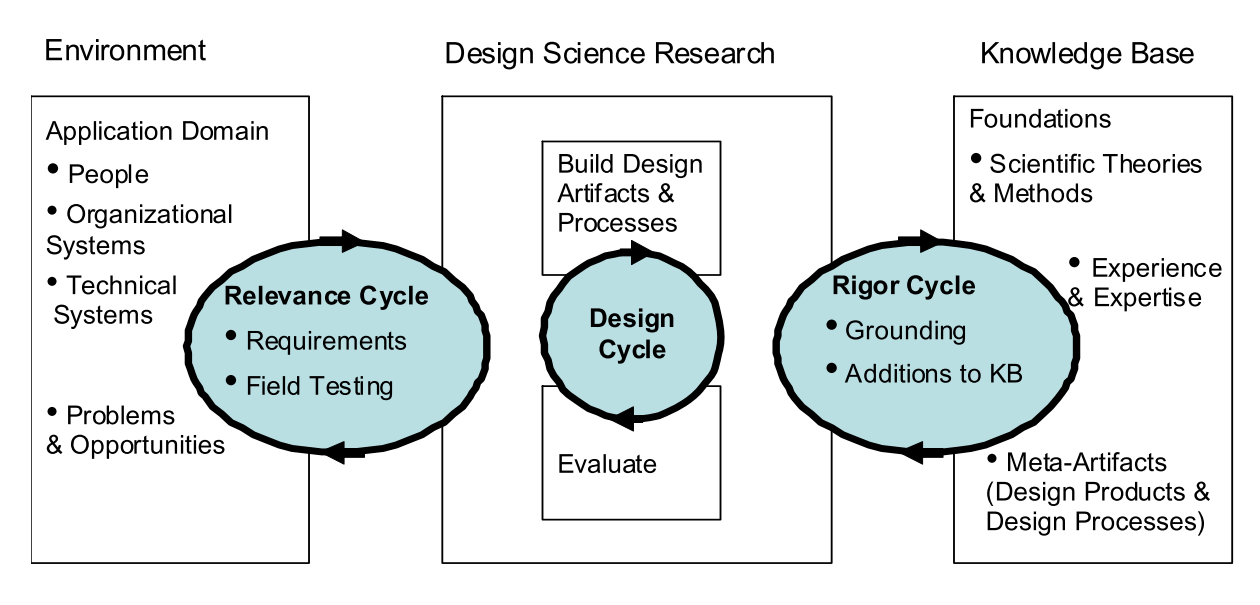
\includegraphics[scale=.24]{Graphics/hevner_DSR.png}
    \vspace*{-8pt}
    \caption{\footnotesize{DSR three cycles from Hevner[3].}}  
  \end{figure}
\end{frame}

\begin{frame}{Methodology}
  \vspace{15pt}
  \emph{Peffers}\cite{Peffers2007} states the research process in six stages. The author specifically proposes a \emph{Design Science Research Methodology} (DSRM). 
  \begin{figure}
    \centering
   \hspace*{-20pt} 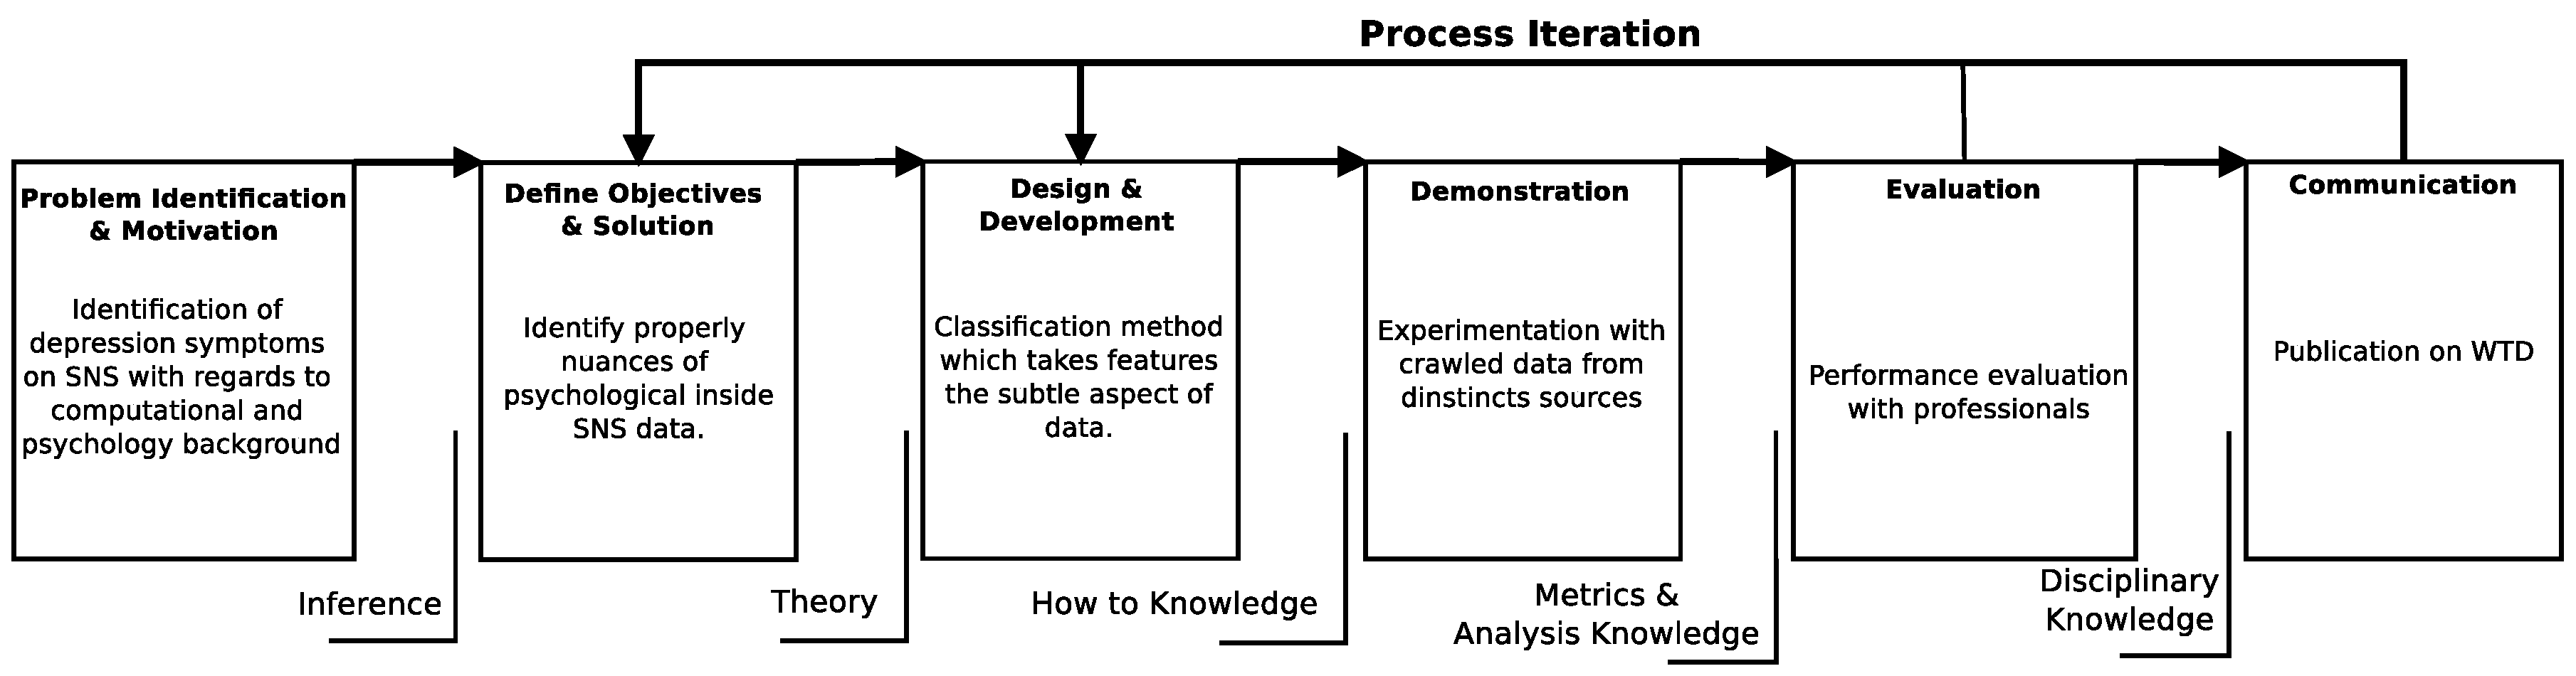
\includegraphics[scale=.25]{Graphics/DSR_Peffer_instance.eps}
    \label{fig:DSR_Peffers_instance}
    \caption{Research stages based on DSRM from \cite{Peffers2007}.}
  \end{figure}
\end{frame}

\begin{frame}{Methodology}
  \begin{block}{}
    % In order to fullfill the components and create the proposed artifact in DSR instatiation,
    We establish which cycles will comprehend each component to fullfill DSR requirements. Taking into account Wieringa approach \cite{Wieringa2014}.

    \begin{itemize}
      \item Systematic Literature Review - Related to Empirical Cycle
      \item Experiments to test and validate initial classification models - Related to Design/Engineering Cycle.
    \end{itemize}
  \end{block}
\end{frame}
%-------------------------------------------------------

\section{1st Cycle}
\subsection{Systematic Literature Review}

\begin{frame}{Research Questions}
  \begin{itemize}
    \item Is it possible to identify symptoms of psychological diseases on social media platforms? % Seria possivel identificar sintomas de doencas psicologicas por meio das midias sociais? 
    \item Is there a diagnosis method which only uses social media data? % Haveria uma forma de diagnosticar um distúrbio usando apenas informacoes das MS? 	
    \item Would the social media platform be useful for professionals? % Seriam as MS's uteis para profissionais, psicologos etc? 	
    \item Assuming there exist such methods, which type of techniques are used on them? % Que tipos de tecnicas de analise poderiam ser utilizadas para tal? 	
    \item % Quando e onde os trabalhos tem sido publicados? 	
    \item What and how is composed the state of the art? % Quais são os trabalhos existentes atuais que abordam depressão? 
  \end{itemize}
\end{frame}

\begin{frame}{Systematic Literature Review}
  \begin{block}{}
    Still in progress.
    \begin{itemize}{}
      \item (“Social Media” OR “Social Network” OR “Complex Network”) AND (Depression OR “Major Depressive Disorder”)
      \item 2013 $\geq$ \textit{published} $\leq$ 2018
      \item 22 from ACM and 25 from IEEE bases
    \end{itemize}
  \end{block}


  \begin{center}
    \begin{table}[h!]
    \centering
    \resizebox{.7\columnwidth}{!}{
      \begin{tabular}{c|c}
        \textbf{Inclusion}          & \textbf{Exclusion}                      \\ \hline
        Directly tackles depression & Out of 2013-2018 scope                  \\ %\hline
        Have computational approach & Not written in english or portuguese    \\ %\hline
        Attend both approaches      & It is not a primary study               \\ %\hline
        -                           & It does not have abstract               \\ %\hline
        -                           & It does not have computing contribution \\ %\hline
        -                           & It has less than 4 pages                \\ %\hline
      \end{tabular}}
      \caption{SLR criteria for inclusion and exclusion.}
      \label{tab:rslCriterias}
    \end{table}
  \end{center}

\end{frame}

\begin{frame}{Systematic Literature Review}
  \begin{block}{}
    \textit{Chen et al.} have detected eight basic emotions and calculated the overall intensity (strength score) of the emotions extracted from all past tweets of each user\cite{Chen2018}.  
  \end{block}
    
  \begin{block}{\small{Approach:}}
    \begin{itemize}
      \item “...identify users with or at risk of depression by incorporating measures of eight basic emotions as features from Twitter posts over time, including a temporal analysis of these features.”
      \item Data obtained from expressions: "I was/have been diagnosed with depression."  
      \item Contributions:
            \begin{itemize}
              \item[$\circ$] Emotions are the analyzed features
              \item[$\circ$] Data analysis over time
              \item[$\circ$] Explore how time series analysis can help on task of identify depressive users
            \end{itemize}
      \item Features:
      \begin{itemize}
        \item[$\circ$] Non-temporal: 9 entries emotion feature vector (emotions + Emotion Overall Score)        
        \item[$\circ$] Temporal: Timestamp for each emotion score 
      \end{itemize}
    \end{itemize}    
  \end{block}
\end{frame}

\begin{frame}{Systematic Literature Review}
  \begin{block}{}
    \textit{Vedula and Parthasarathy} conduct an observational study to understand the interactions between clinically depressed users and their ego-network when contrasted with a group of users without depression. They identify relevant linguistic and emotional signals from social media exchanges to detect symptomatic cues of depression\cite{Vedula2017}.
  \end{block}

  \begin{block}{\small{Approach:}}
    Examine network effects related to:
    \begin{itemize}
      \item participation (passive: tweets a user is exposed to, retweets or mentions a user receives; active: mentions, retweets and conversations made by the user)
      \item engagement (content (e.g., linguistic cues, emotion) and relational dynamics (e.g., conflict/support, influence))
      \item Ego-neighborhood (size, centrality and affinity to form clusters or communities)
    \end{itemize}
  \end{block}
\end{frame}

\begin{frame}{Systematic Literature Review}
  \begin{block}{}
    \textit{De Choudhury et al.} have used crowdsourcing to obtain data from twitter by people who were clinically diagnosed with depression. They also have constructed a corpus and developed a probabilistic model. The trained model classifies if a post indicates depression\cite{DeChoudhury:2013:SMM:2464464.2464480}. Similarly, \textit{ et al} have applied the same analysis to replicate the results in a group of japanese users\cite{Tsugawa2015}.
  \end{block}{}

  \begin{block}{}
    \begin{itemize}
      \item Problem:
        \begin{itemize}
          \item[$\circ$] Characterize levels of depression in populations.          
        \end{itemize}
      \item Approach:
        \begin{itemize}
          \item[$\circ$] Crowdsourcing to build a large corpus of postings on Twitter that have been shared by individuals diagnosed with clinical depression.
          \item[$\circ$] Probabilistic model trained on this corpus to determine if posts could indicate depression
          \item[$\circ$] Social media depression index that may serve to characterize levels of depression in populations
        \end{itemize}
    \end{itemize}
  \end{block}
\end{frame}

\begin{frame}{Systematic Literature Review}
    % Please add the following required packages to your document preamble:
        \begin{table}
        \vspace*{3pt}
        \hspace*{-.5cm}
        \centering
        \resizebox{.93\paperwidth}{!}{%
            % \begin{tabular}{c|c|c|c|c|c}
            \begin{tabular}{c|c|c|c|c|c}
    
            \textbf{Reference} & \textbf{Method/Model/Algorithm} & \textbf{Features} &\begin{tabular}[c]{@{}c@{}} \textbf{Psychological}\\ \textbf{Approach} \end{tabular} & \textbf{Dataset} & \begin{tabular}[c]{@{}c@{}} \textbf{Behaviour}\\ \textbf{Variation} \end{tabular}\\ \hline % & \textbf{Contribution} \\ \hline
            %  2018
            \cite{trotzek_utilizing_2018} & CNN - CReLU & LIWC &  & CLEF e-Risk(Reddit) & No \\ \hline
            
            \cite{wongkoblap_multilevel_2018} & SVM w/ RBF kernel; PCA & \begin{tabular}[c]{@{}c@{}}LIWC, demography, \\ activities, post time\end{tabular} & CES-D & Facebook myPersonality & Yes$\dagger$% \multicolumn{1}{c}{\begin{tabular}[c]{@{}c@{}}Analyze correlation between life satisfaction\\  and depression among SNS users; \\ multilevel predictive model to \\ detect users with depression\end{tabular}} 
            \\ \hline
            
            \cite{silveira_fraga_online_2018} & RMN? &  &  & Reddit & Yes$\dagger$\\ \hline
    
            \cite{katchapakirin_facebook_2018} & SVM, RF, DL* & \begin{tabular}[c]{@{}c@{}} Information about generated content \\ (content, interactions, privacy and behavior) \end{tabular} & TMHQ & Facebook Users volunteers & No\\ \hline % & new psychological instrument \\ \hline
    
            \cite{oyong_natural_2018} & \begin{tabular}[c]{@{}c@{}} NLP \\(lexical construction approach)\end{tabular} &  & CES-D for lexical construction & Filtered Tweets & No \\ \hline

            \cite{murtagh_analysing_2018} & Undefined & Undefined &&& \\ \hline
          
            % 2017
            % \cite{calderon-vilca_simulation_2017} & data simulation &&& & \\ \hline %& Not Related \\ \hline
            
            \cite{simms_detecting_2017} & Logistic Regression & subset processed from LIWC & Professional Validation & Tumblr API & No \\ \hline
    
            % \cite{zucco_sentiment_2017} $\dagger$  & &&& \\ \hline % & Does not bring contribution \\ \hline
    
            % \cite{noureen_semantic_2017} $\dagger$ & &&& \\ \hline %& Does not bring contribution \\ \hline
    
            % 2016
            \cite{akay_assessing_2016} & Weighted Network Model, NLTK, SNA & & & depressionforums.org & No\\ \hline
    
            \cite{saha_framework_2016} & Own Method & LIWC, LDA & & LiveJournal.com & No\\ \hline
    
            \cite{dao_effect_2016} & Lasso & ANEW, LIWC, LDA & & LiveJournal & No\\ \hline
    
            \cite{dao_discovering_2016} & Non-Negative Matrix Factorization & ANEW & & LiveJournal& No\\ \hline
    
            % 2015
            \cite{dao_nonparametric_2015} & Nonparametric Clustering, Hierarchical Dirichlet & ANEW, LDA && LiveJournal.com & No\\ \hline
          
            \cite{chomutare_mining_2015} & BoW &&& Undefined source& No\\ \hline
    
            \cite{nambisan_social_2015} & Hypothesis Test &&& Filtered Tweets & No\\ \hline
    
            \cite{larsen_we_2015} & PCA(not main) & ANEW, LIWC, Tweet metadata, timezone & & Filtered Tweets & Yes$\dagger$\\ \hline
    
            % 2014
            \cite{nguyen_affective_2014} & Lasso & ANEW, LIWC, LDA && LiveJournal.com & No\\ \hline
    
            \cite{fang_mental_2014} & Quant. Analysis & Depression Ontology & & & Yes$\dagger$\\ \hline
    
            \cite{dao_analysis_2014} & Quant. and Behaviour Analysis & Sentiment and Linguistic(LIWC), ANEW & & LiveJournal & Yes$\star$\\ \hline
    
            % % 2013
            \cite{wang_improved_2013} & Decision Tree & Relationship's Topology & & Sina Micro-blog & No\\
    
            % \cite{li_content_2013} $\dagger$ & & & &
    
          \end{tabular}%
            }
            \caption{\scriptsize{Review of Literature approaches from IEEE. Where $\dagger$ stands papers where analysis over time were made but not used in model creation task, consequently $\star$ stands for the inverse.}}
            \label{tab:IEEE_papers}
        \end{table}
      \end{frame}


  \begin{frame}{Systematic Literature Review}
    % Please add the following required packages to your document preamble:
        \begin{table}
        \vspace*{-.15cm}
        \centering
        \resizebox{.8\paperwidth}{!}{%
        
            % \begin{tabular}{c|c|c|c|c|c}
            \begin{tabular}{c|c|c|c|c|c}
    
            \textbf{Reference} & \textbf{Method/Model/Algorithm} & \textbf{Features} & \begin{tabular}[c]{@{}c@{}}\textbf{Psychological}\\ \textbf{Approach} \end{tabular} & \textbf{Dataset} & \begin{tabular}[c]{@{}c@{}} \textbf{Behaviour}\\ \textbf{Variation} \end{tabular} \\ \hline % & \textbf{Contribution} \\ \hline
            % 2013
            \cite{DeChoudhury:2013:PPC:2470654.2466447} &SVM w/ kernel &\begin{tabular}[c]{@{}c@{}} Engagement(avg. n. of posts, replies and retweets),\\ Ego-Network(n. of followers and followees),\\ Polarity Emotion(LIWC and ANEW), Linguistic(LIWC)\end{tabular}&& Twitter & \\ \hline
            \cite{DeChoudhury:2013:SMM:2464464.2464480} & SVM & \begin{tabular}[c]{@{}c@{}} Post Features(Emotion, Time, Ling., n-grams)\\ User Features(n. of posts, replies and retweets)\end{tabular} & CES-D & Twitter and Crowdsourcing  & Yes$\dagger$\\ \hline 
            \cite{de_choudhury_major_2013} &Quant. and Qual. Analysis & \begin{tabular}[c]{@{}c@{}} \\Activity(n. of posts), Emotion(LIWC) \\Linguistic(LIWC)\end{tabular}& & Twitter and Crowdsourcing & Yes\\ \hline

            % 2014
            \cite{Homan:2014:SSD:2531602.2531704} & Quant. and Qual. Analysis & Network components(degree, triangles, clustering) & PHQ-9 & TrevorSpace & No \\ \hline
            \cite{Wilson:2014:FIM:2637002.2637006} & Qual. and Linguistic Analysis & LIWC & & Twitter & No\\ \hline
            
            % 2015
            \cite{Park:2015:MDL:2675133.2675139} & Quant. and Qual. Analysis & \begin{tabular}[c]{@{}c@{}} Profile, Application and Posts Activities,\\Likes and Comments Interactions,\\Perceived Mood \end{tabular}& CES-D & Faceboook App & Yes$\dagger$\\ \hline
            \cite{Tsugawa2015} & SVM w/ kernel & \begin{tabular}[c]{@{}c@{}} BoW, LDA, Sent. Ratio,\\tweet metadata, n. of following and followers\end{tabular}  & CED-D & Twitter & \\ \hline
            
            % 2016
            \cite{Kavuluru:2016:CHC:2975167.2975170} & linear SVM & N-grams, LIWC, discourse relation graph & Professional Validation & Reddit subgroup & No \\ \hline
            \cite{Li2016} & Qualitative Analysis & & & SunForum & No\\ \hline
            
            % 2017 
            \cite{DeChoudhury:2017:GCD:2998181.2998220} & & \begin{tabular}[c]{@{}c@{}} \end{tabular} & Twitter & &\\ \hline
            \cite{Vedula2017} & Gradient Boosted DT + CV & topology, social media metadata & CES-D & Twitter(API) & Yes$\star$ \\ \hline
            \cite{andalibi_sensitive_2017} & Qualitative analysis & & & Instagram(API) & No\\ \hline
            \cite{Yazdavar:2017:SAM:3110025.3123028} &  \begin{tabular}[c]{@{}c@{}} Topic Identification,\\ Sent. Analysis,\\ Multi-Label Classification\end{tabular} & LDA, Lexicon(depression related terms) & PHQ-9 & Twitter & Yes$\star$\\ \hline
            \cite{Bagroy:2017:SMB:3025453.3025909} & & & & Reddit & Yes\\ \hline
            
            % 2018
            \cite{Nobles:2018:IIS:3173574.3173987} & SVM and LIWC & LIWC and word occurrence & & \begin{tabular}[c]{@{}c@{}} (SMS and email), Facebook, Twitter\\ web browsing history,\\ mental health history \end{tabular} & No \\ \hline
            \cite{Chen2018} & (SVM, RF) + CV &\begin{tabular}[c]{@{}c@{}} Emotive(Ontology), Temporal,\\ Non-temporal(emotions vectors), LIWC \end{tabular}& & Twitter & Yes$\star$\\ \hline

            \cite{Sadeque2018} & \begin{tabular}[c]{@{}c@{}} Non-Sequential(SVM),\\Sequential Model(RNN)\end{tabular} & Words, DepWords, DepEmbed, MetaMap & & CLEF eRisk 2017 & No \\ \hline
            \cite{Zhao:2018:TCM:3302425.3302501} & Double Input CNN & Text (Semantic Content) \& External (Text Characterization) & & Tree Hole & No \\ \hline

        \end{tabular}%
        }
        \caption{\scriptsize{Review of Literature approaches from ACM. Where $\dagger$ stands papers where analysis over time were made but not used in model creation task, and $\star$ stands for the inverse.}}
        \label{tab:ACM_papers}
        \end{table}
  \end{frame}

\begin{frame}
  \begin{itemize}
    \item Análise Textual
      \ Identificação de emoções/sentimentos
    Assuntos abordados
    … (completar)
    \item Conteúdo
    Horário da postagem
    Local
    Privacidade do conteúdo
    … (completar)
    \item Perfil do Usuário
    Gênero
    Local
    Idade
    Estado do Relacionamento (por exemplo: solteiro)
    … (completar)
    \item Comportamental (do usuário perante a plataforma)
    Quantidade de mudanças do estado do relacionamento
    Horário que fica online
    … (completar)
    \item Interação com Outros
    Número de grupos que participa
    Número de fotos onde foi marcado
    Quantidade de amigos 
    Quantidade de seguidos/seguidores
    … (completar)
    Métricas de redes sociais referentes ao nó (por exemplo, grau do nó)
    … (completar)
    \item Características do grupo 
    Métricas de redes sociais referentes ao grupo (por exemplo, densidade, modularidade, etc.)
    … (completar)
    \item Variação Longitudinal (Variação ao longo do tempo)
    Sim/Não
    Período (sazionalidade)
    
  \end{itemize}
\end{frame}

\begin{frame}{Literature Gaps}
  \begin{itemize}
    \item Not all the analyzed researches take into account the psychology point of view. 
    \item Use of psychometrics only
    \item Would the screening of depressive users be more robust and reliable if they take others psychology approaches?
    \item Is it possible to identify the same symptoms from clinical using computational techniques?
    \item Aggregated Data Analysis vs Individual Data Analysis
  \end{itemize}
\end{frame}

\section{2nd Cycle}
\subsection{Contribution Proposal}

\begin{frame}{Contribution Proposal}
  \begin{figure}
    \centering
    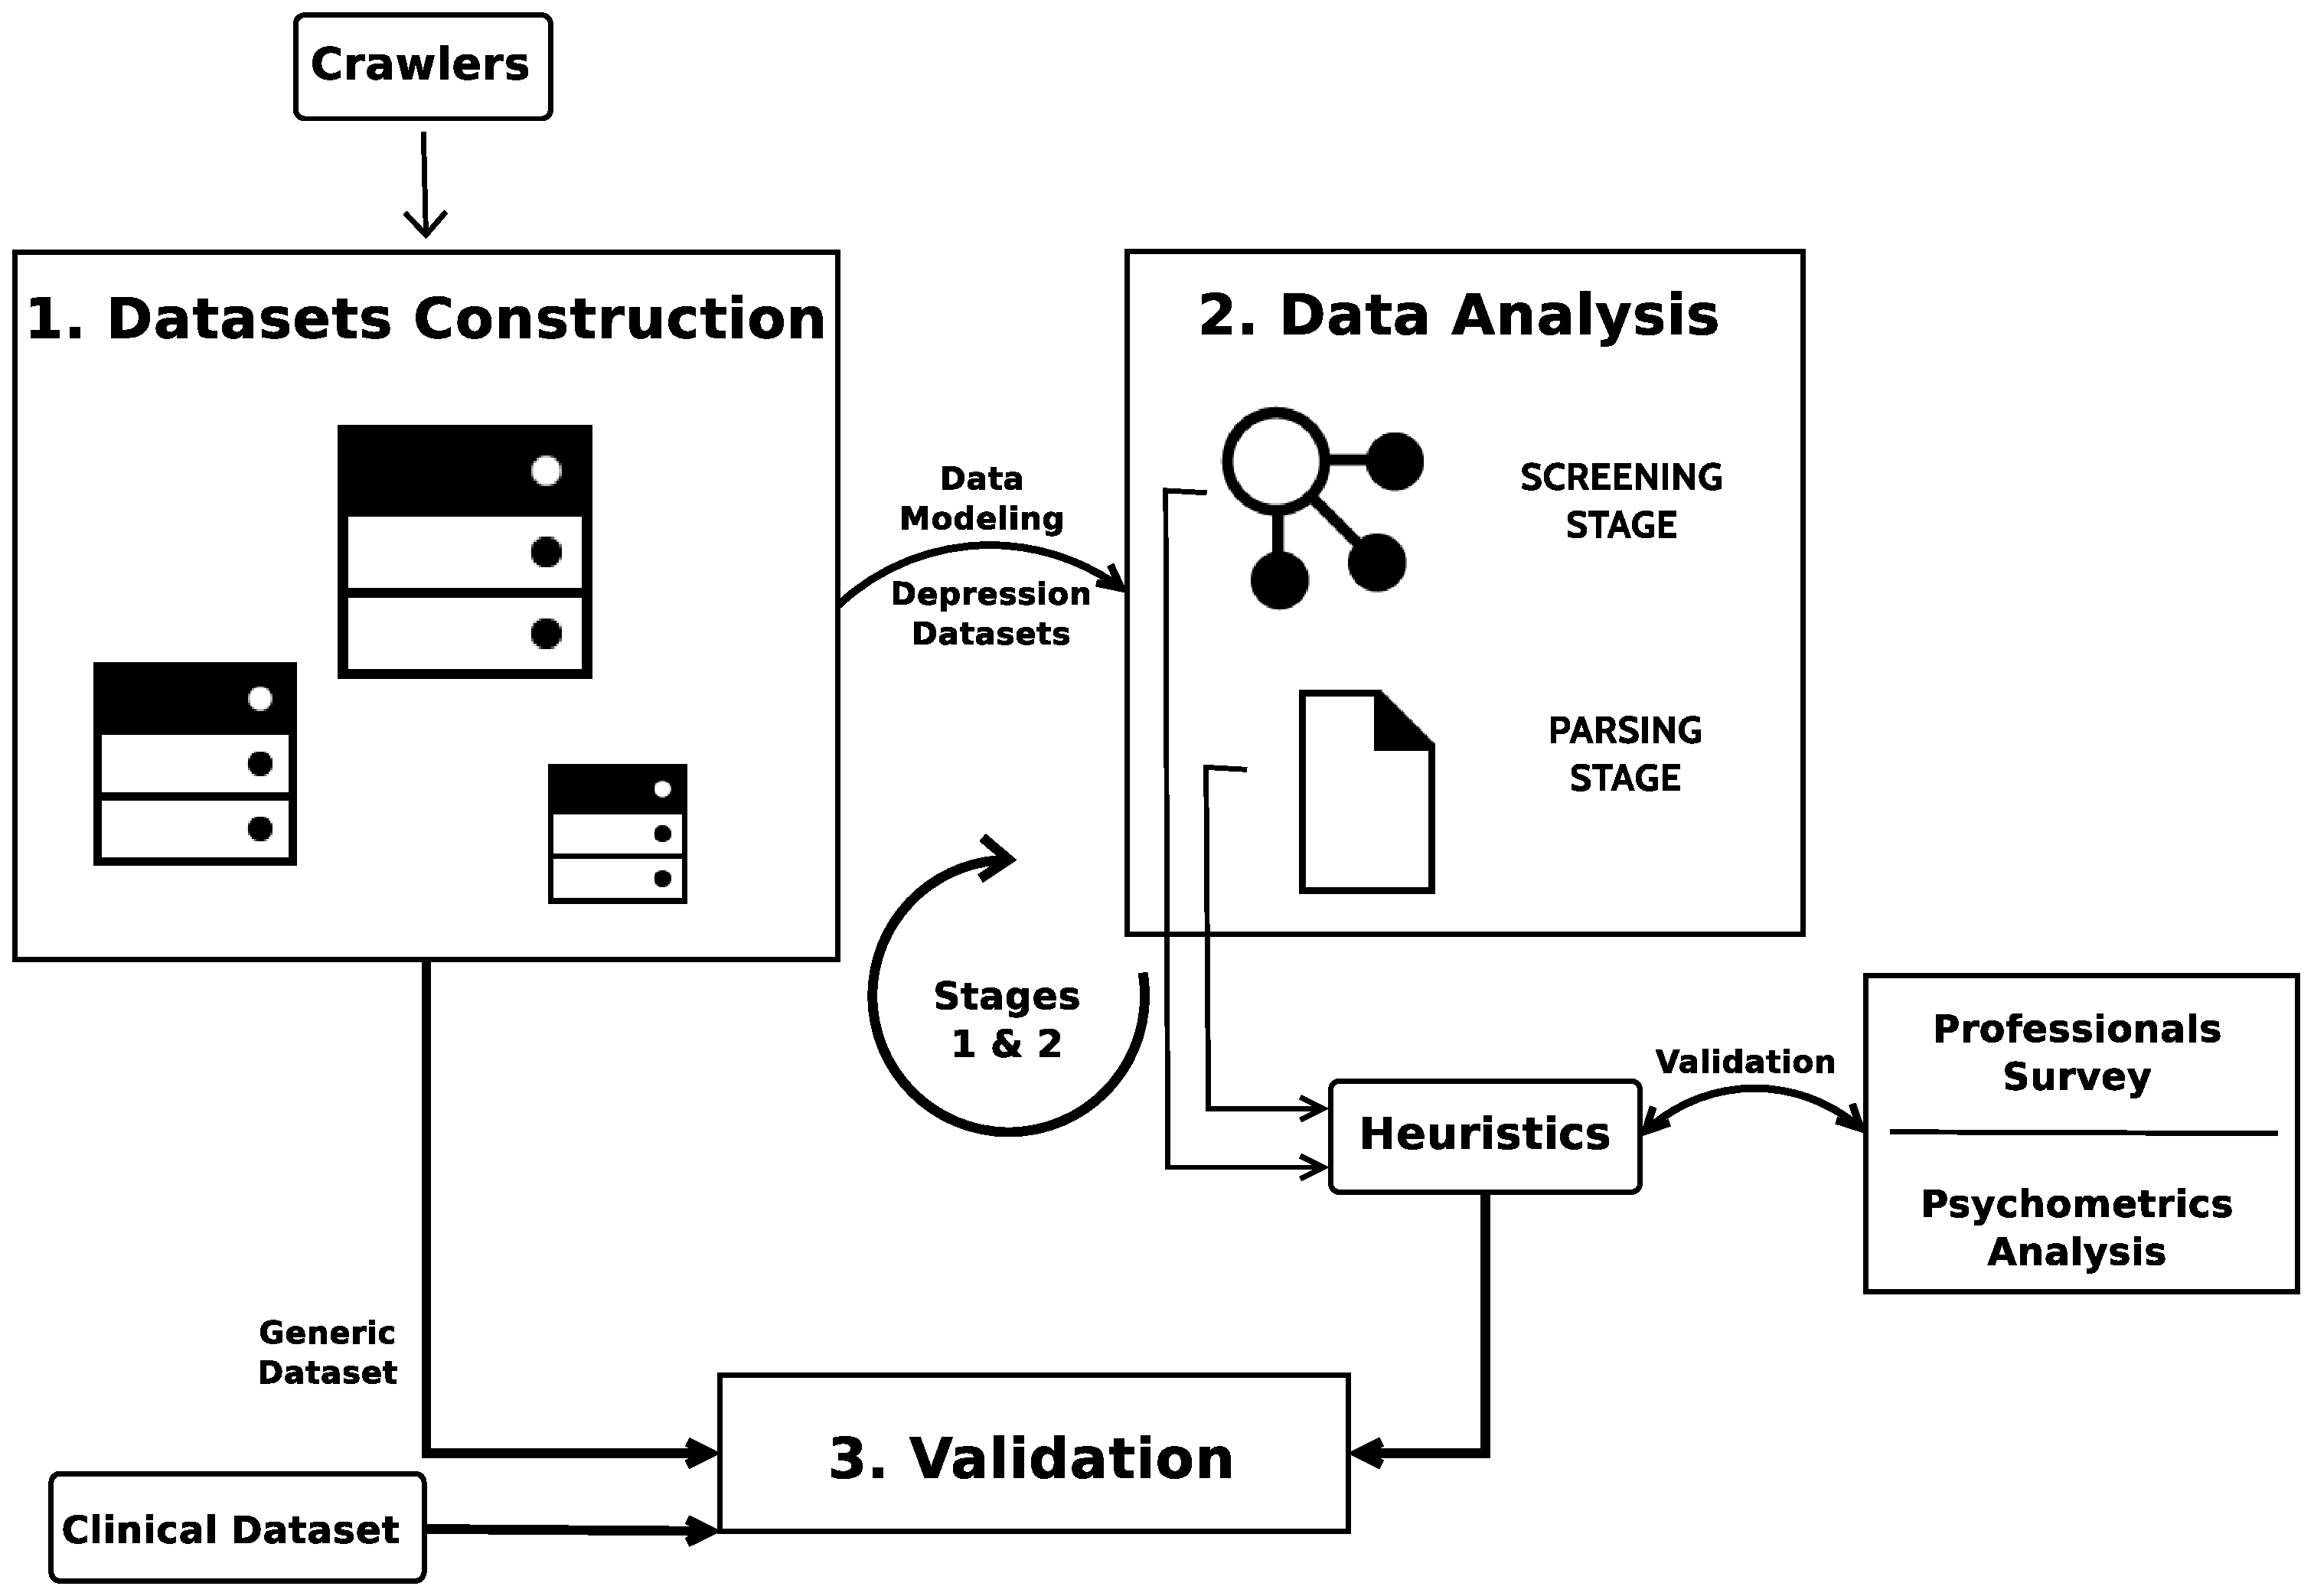
\includegraphics[scale=.175]{Graphics/conceptualModel.eps}
    \caption{\small{Proposal Conceptual Model}}
    \label{fig:conceptualModel}
  \end{figure}
\end{frame}

\subsection{Technical Challenges}
\begin{frame}{Technical Challenges}
  \begin{itemize}
    \item Validation with clinical data
    \item Datasets to train classification model
    \item Reliable data, taking into account people consent
    \item Improve Computer Science area
  \end{itemize}
\end{frame}

% \section{DSR Instantiation}
% \begin{frame}{DSR Instantiation}
%     \begin{figure}
%       \centering
%       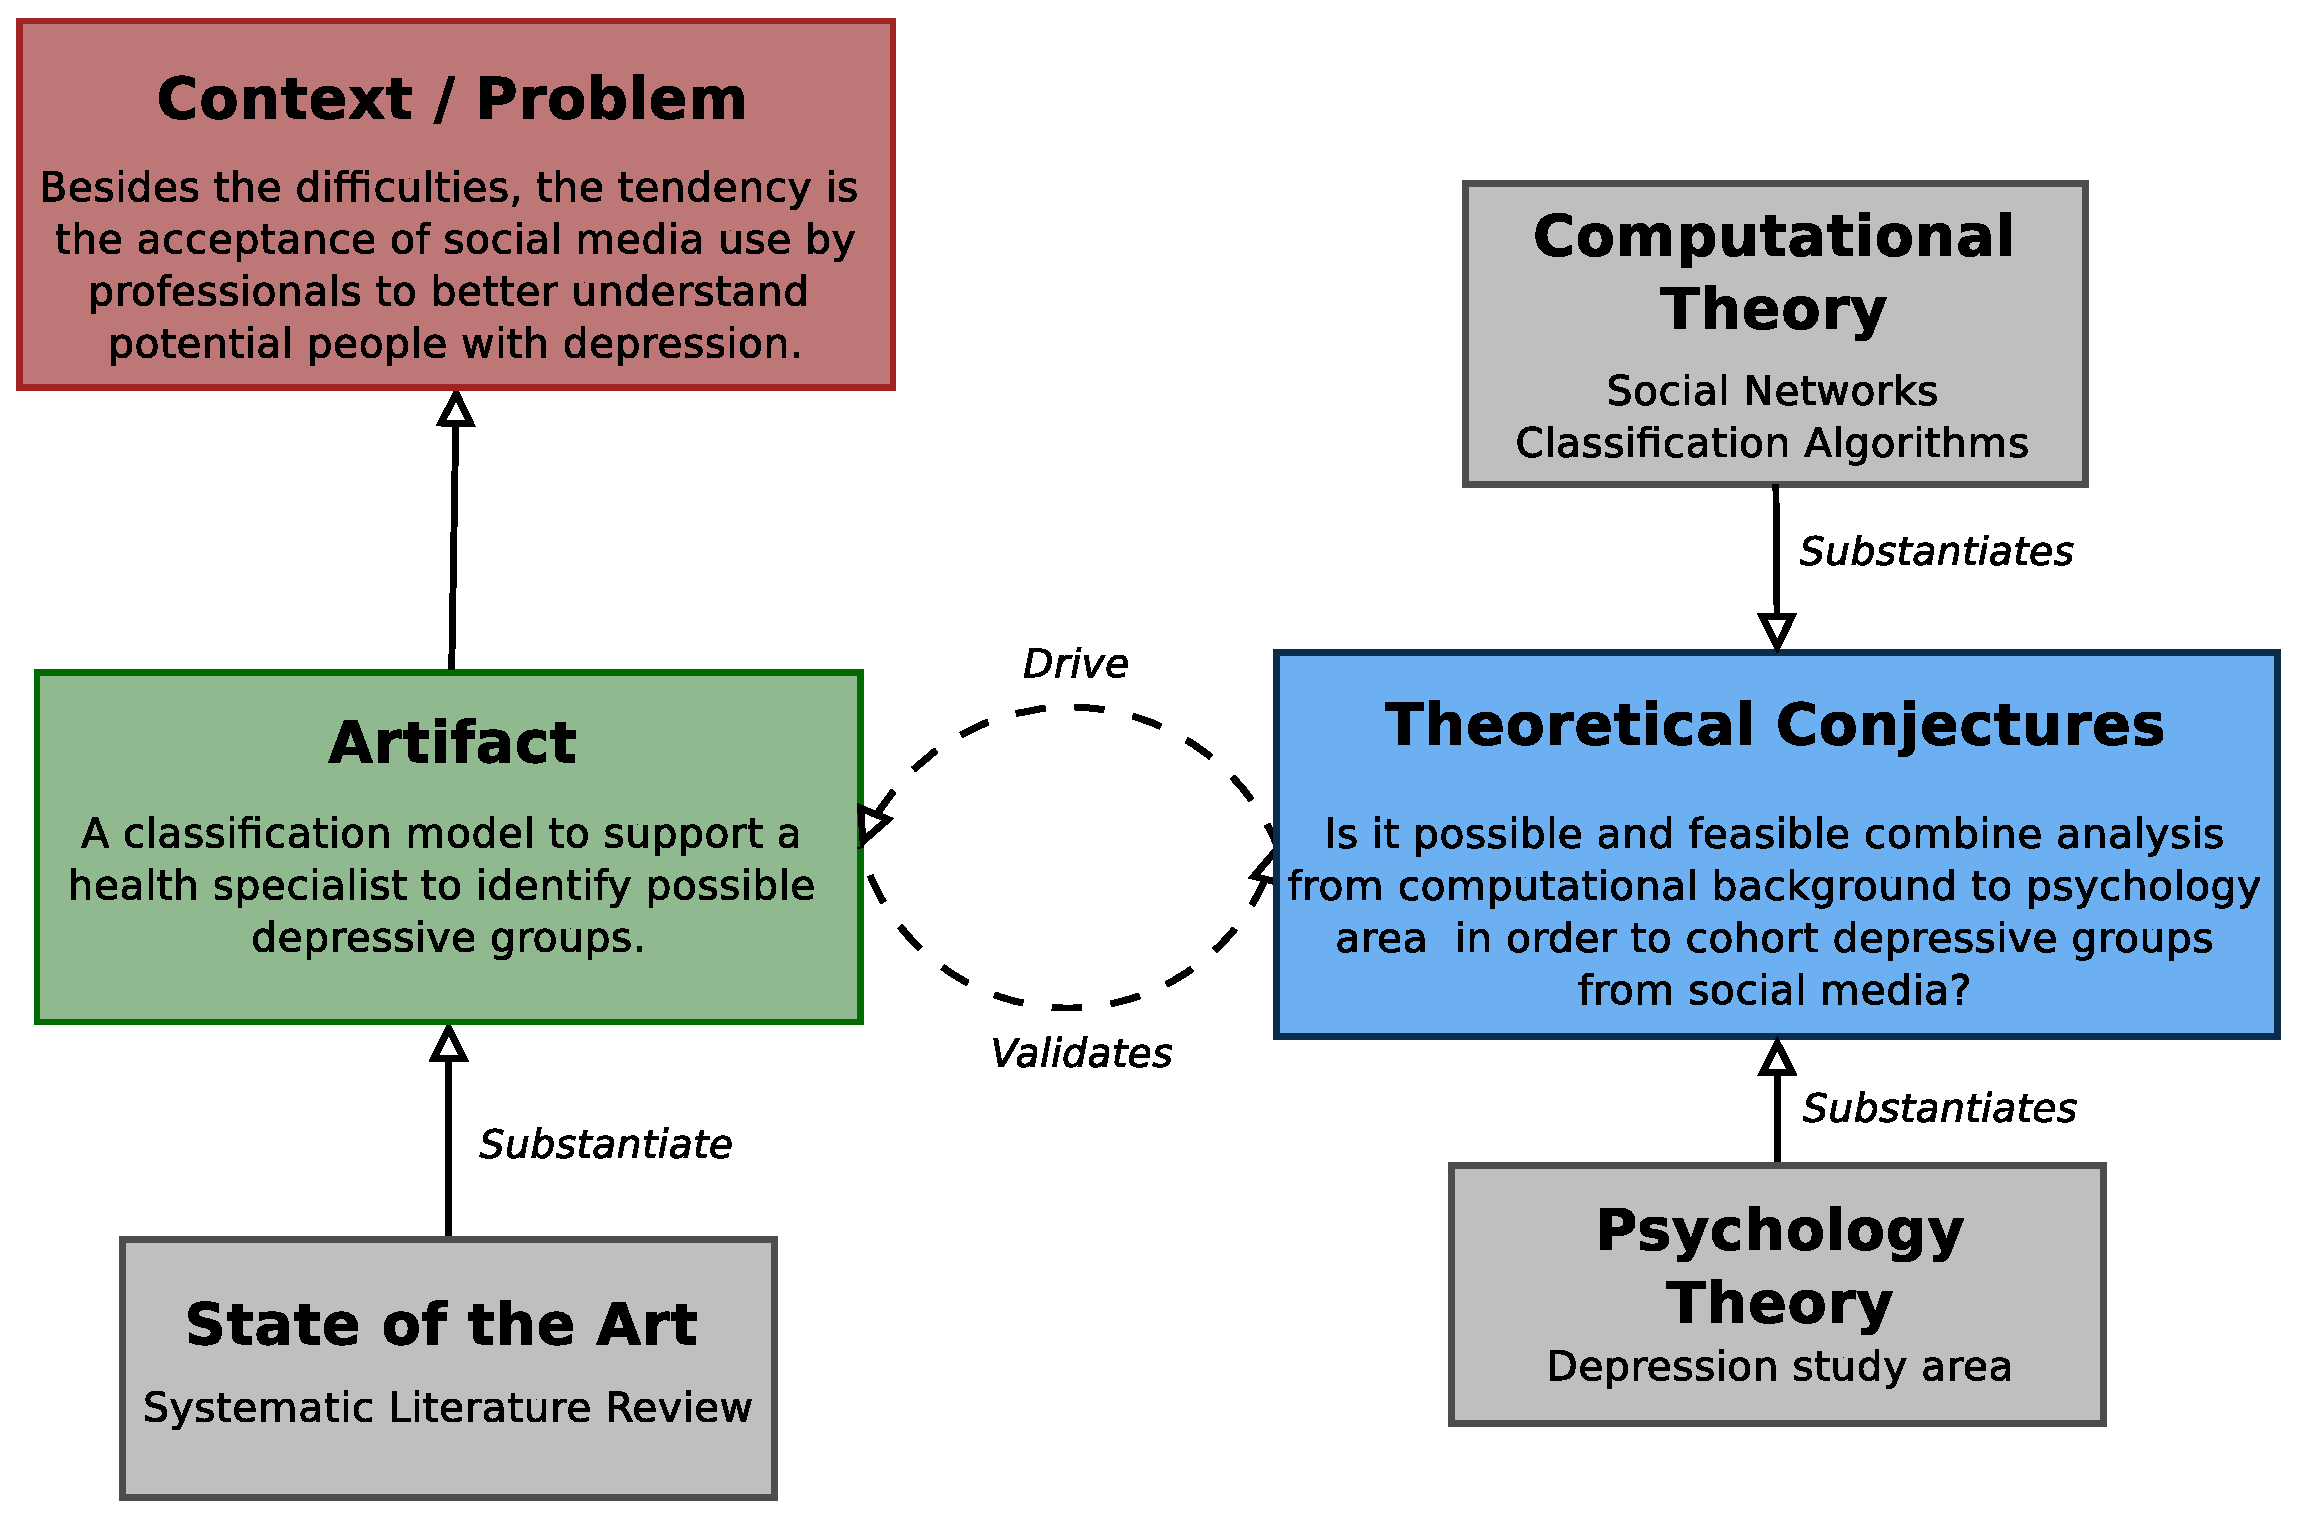
\includegraphics[scale=.3]{Graphics/DSR_diagram.eps}
%       \label{fig:DSR_proposal}
%       \caption{\footnotesize DSR instantiation.}
%     \end{figure}
  
%   \end{frame}
  

  
\section{Future Steps}
\begin{frame}{Schedule}
  \begin{itemize}
    \item Submission to WTD on SBBD (08/07)
    \item Proposal writing - In progress - First issue 15/07
    \item Qualification - End of August
    \item Ending of 1st Cycle
    \item Ending of 2nd Cycle
  \end{itemize}
\end{frame}

\begin{frame}{Backup}{Abstraction of Studies} - BE INCLUDED
    1) Classificação dos trabalhos encontrados no mapeamento, ressaltando: Objetivo do trabalho, Abordagem utilizada, Técnicas utilizadas (algoritmos e métricas), Principais desafios levantados (ou trabalhos futuros). 
    
  
    2) A partir do material que vc. leu, destacar o conjunto de teorias/referências que vão embasar o seu problema e a sua motivação (Conjecturas Teóricas)
    
    
    3) Quadro explicativo, com as métricas/features que os trabalhos relacionados usam e as métricas/features que vc. pensou em incluir na sua proposta. Este quadro deve ter: o nome da métrica/feature, explicação sucinta sobre a métrica/feature, referência (ao trabalho que a usou), justificativa do seu uso. 
    
  \end{frame}



  \begin{frame}{Systematic Literature Review}
    % Please add the following required packages to your document preamble:
        \begin{table}
        \vspace*{3pt}
        \hspace*{-.5cm}
        \centering
        \resizebox{.93\paperwidth}{!}{%
            % \begin{tabular}{c|c|c|c|c|c}
            \begin{tabular}{c|c|c|c|c|c}
    
            \textbf{Reference} & \textbf{Method/Model/Algorithm} & \textbf{Features} &\begin{tabular}[c]{@{}c@{}} \textbf{Psychological}\\ \textbf{Approach} \end{tabular} & \textbf{Dataset} & \begin{tabular}[c]{@{}c@{}} \textbf{Behaviour}\\ \textbf{Variation} \end{tabular}\\ \hline % & \textbf{Contribution} \\ \hline
            %  2018
            \cite{trotzek_utilizing_2018} & CNN - CReLU & LIWC &  & CLEF e-Risk(Reddit) & No \\ \hline
            
            \cite{wongkoblap_multilevel_2018} & SVM w/ RBF kernel; PCA & \begin{tabular}[c]{@{}c@{}}LIWC, demography, \\ activities, post time\end{tabular} & CES-D & Facebook myPersonality & Yes$\dagger$% \multicolumn{1}{c}{\begin{tabular}[c]{@{}c@{}}Analyze correlation between life satisfaction\\  and depression among SNS users; \\ multilevel predictive model to \\ detect users with depression\end{tabular}} 
            \\ \hline
            
            \cite{silveira_fraga_online_2018} & RMN? &  &  & Reddit & Yes$\dagger$\\ \hline
    
            \cite{katchapakirin_facebook_2018} & SVM, RF, DL* & \begin{tabular}[c]{@{}c@{}} Information about generated content \\ (content, interactions, privacy and behavior) \end{tabular} & TMHQ & Facebook Users volunteers & No\\ \hline % & new psychological instrument \\ \hline
    
            \cite{oyong_natural_2018} & \begin{tabular}[c]{@{}c@{}} NLP \\(lexical construction approach)\end{tabular} &  & CES-D for lexical construction & Filtered Tweets & No \\ \hline

            \cite{murtagh_analysing_2018} & Undefined & Undefined &&& \\ \hline
          
            % 2017
            % \cite{calderon-vilca_simulation_2017} & data simulation &&& & \\ \hline %& Not Related \\ \hline
            
            \cite{simms_detecting_2017} & Logistic Regression & subset processed from LIWC & Professional Validation & Tumblr API & No \\ \hline
    
            % \cite{zucco_sentiment_2017} $\dagger$  & &&& \\ \hline % & Does not bring contribution \\ \hline
    
            % \cite{noureen_semantic_2017} $\dagger$ & &&& \\ \hline %& Does not bring contribution \\ \hline
    
            % 2016
            \cite{akay_assessing_2016} & Weighted Network Model, NLTK, SNA & & & depressionforums.org & No\\ \hline
    
            \cite{saha_framework_2016} & Own Method & LIWC, LDA & & LiveJournal.com & No\\ \hline
    
            \cite{dao_effect_2016} & Lasso & ANEW, LIWC, LDA & & LiveJournal & No\\ \hline
    
            \cite{dao_discovering_2016} & Non-Negative Matrix Factorization & ANEW & & LiveJournal& No\\ \hline
    
            % 2015
            \cite{dao_nonparametric_2015} & Nonparametric Clustering, Hierarchical Dirichlet & ANEW, LDA && LiveJournal.com & No\\ \hline
          
            \cite{chomutare_mining_2015} & BoW &&& Undefined source& No\\ \hline
    
            \cite{nambisan_social_2015} & Hypothesis Test &&& Filtered Tweets & No\\ \hline
    
            \cite{larsen_we_2015} & PCA(not main) & ANEW, LIWC, Tweet metadata, timezone & & Filtered Tweets & Yes$\dagger$\\ \hline
    
            % 2014
            \cite{nguyen_affective_2014} & Lasso & ANEW, LIWC, LDA && LiveJournal.com & No\\ \hline
    
            \cite{fang_mental_2014} & Quant. Analysis & Depression Ontology & & & Yes$\dagger$\\ \hline
    
            \cite{dao_analysis_2014} & Quant. and Behaviour Analysis & Sentiment and Linguistic(LIWC), ANEW & & LiveJournal & Yes$\star$\\ \hline
    
            % % 2013
            \cite{wang_improved_2013} & Decision Tree & Relationship's Topology & & Sina Micro-blog & No\\
    
            % 2013
            \cite{DeChoudhury:2013:PPC:2470654.2466447} &SVM w/ kernel &\begin{tabular}[c]{@{}c@{}} Engagement(avg. n. of posts, replies and retweets),\\ Ego-Network(n. of followers and followees),\\ Polarity Emotion(LIWC and ANEW), Linguistic(LIWC)\end{tabular}&& Twitter & \\ \hline
            \cite{DeChoudhury:2013:SMM:2464464.2464480} & SVM & \begin{tabular}[c]{@{}c@{}} Post Features(Emotion, Time, Ling., n-grams)\\ User Features(n. of posts, replies and retweets)\end{tabular} & CES-D & Twitter and Crowdsourcing  & Yes$\dagger$\\ \hline 
            \cite{de_choudhury_major_2013} &Quant. and Qual. Analysis & \begin{tabular}[c]{@{}c@{}} \\Activity(n. of posts), Emotion(LIWC) \\Linguistic(LIWC)\end{tabular}& & Twitter and Crowdsourcing & Yes\\ \hline

            % 2014
            \cite{Homan:2014:SSD:2531602.2531704} & Quant. and Qual. Analysis & Network components(degree, triangles, clustering) & PHQ-9 & TrevorSpace & No \\ \hline
            \cite{Wilson:2014:FIM:2637002.2637006} & Qual. and Linguistic Analysis & LIWC & & Twitter & No\\ \hline
            
            % 2015
            \cite{Park:2015:MDL:2675133.2675139} & Quant. and Qual. Analysis & \begin{tabular}[c]{@{}c@{}} Profile, Application and Posts Activities,\\Likes and Comments Interactions,\\Perceived Mood \end{tabular}& CES-D & Faceboook App & Yes$\dagger$\\ \hline
            \cite{Tsugawa2015} & SVM w/ kernel & \begin{tabular}[c]{@{}c@{}} BoW, LDA, Sent. Ratio,\\tweet metadata, n. of following and followers\end{tabular}  & CED-D & Twitter & \\ \hline
            
            % 2016
            \cite{Kavuluru:2016:CHC:2975167.2975170} & linear SVM & N-grams, LIWC, discourse relation graph & Professional Validation & Reddit subgroup & No \\ \hline
            \cite{Li2016} & Qualitative Analysis & & & SunForum & No\\ \hline
            
            % 2017 
            \cite{DeChoudhury:2017:GCD:2998181.2998220} & & \begin{tabular}[c]{@{}c@{}} \end{tabular} & Twitter & &\\ \hline
            \cite{Vedula2017} & Gradient Boosted DT + CV & topology, social media metadata & CES-D & Twitter(API) & Yes$\star$ \\ \hline
            \cite{andalibi_sensitive_2017} & Qualitative analysis & & & Instagram(API) & No\\ \hline
            \cite{Yazdavar:2017:SAM:3110025.3123028} &  \begin{tabular}[c]{@{}c@{}} Topic Identification,\\ Sent. Analysis,\\ Multi-Label Classification\end{tabular} & LDA, Lexicon(depression related terms) & PHQ-9 & Twitter & Yes$\star$\\ \hline
            \cite{Bagroy:2017:SMB:3025453.3025909} & & & & Reddit & Yes\\ \hline
            
            % 2018
            \cite{Nobles:2018:IIS:3173574.3173987} & SVM and LIWC & LIWC and word occurrence & & \begin{tabular}[c]{@{}c@{}} (SMS and email), Facebook, Twitter\\ web browsing history,\\ mental health history \end{tabular} & No \\ \hline
            \cite{Chen2018} & (SVM, RF) + CV &\begin{tabular}[c]{@{}c@{}} Emotive(Ontology), Temporal,\\ Non-temporal(emotions vectors), LIWC \end{tabular}& & Twitter & Yes$\star$\\ \hline

            \cite{Sadeque2018} & \begin{tabular}[c]{@{}c@{}} Non-Sequential(SVM),\\Sequential Model(RNN)\end{tabular} & Words, DepWords, DepEmbed, MetaMap & & CLEF eRisk 2017 & No \\ \hline
            \cite{Zhao:2018:TCM:3302425.3302501} & Double Input CNN & Text (Semantic Content) \& External (Text Characterization) & & Tree Hole & No \\ \hline

        \end{tabular}%
        }
        \caption{\scriptsize{Review of Literature approaches from ACM. Where $\dagger$ stands papers where analysis over time were made but not used in model creation task, and $\star$ stands for the inverse.}}
        \label{tab:ACM_papers}
        \end{table}
  \end{frame}

%-------------------------------------------------------
% \subsection{Local and Global installation}
% \begin{frame}{Installation}{Local and Global installation}
% %-------------------------------------------------------
%   The theme can be installed for \textbf{local} or \textbf{global} use.
%   \pause
%   \begin{block}{Local Installation}
%   \begin{itemize}    
%     \item Local installation is the simplest way of installing the theme. 
%     \item You need to placing the 4 source files in the same folder as your presentation. When you download the theme, the 4 theme files are located in the {\tt local} folder.
%   \end{itemize}
%   \end{block}

%   \begin{block}{Global Installation}
%   \begin{itemize}
%      \item If you wish to make the theme globally available, you must put the files in your local latex directory tree. The location of the root of the local directory tree depends on your operating system and the latex distribution. 
%      \item Detailed steps on how to proceed installation under various operating systems can be found at Beamer documentation.
%   \end{itemize}
%   \end{block}
% \end{frame}
     

% %-------------------------------------------------------
% \subsection{Required Packages}
% \begin{frame}{Installation}{Required Packages}
% %-------------------------------------------------------

%   For using the Feather Theme you will need the Bemaer class installed and the following 2 packages
%   \begin{itemize}
%     \item TikZ\footnote{TikZ is a package for creating beautiful graphics. Have a look at these \chref{http://www.texample.net/tikz/examples/}{online examples} or the \chref{http://tug.ctan.org/tex-archive/graphics/pgf/base/doc/generic/pgf/pgfmanual.pdf}{pgf user manual}.}
%     \item calc
%   \end{itemize}
%   Due to the fact that the packages are very common they should be included in your latex distribution in the first place.
% \end{frame}

% %-------------------------------------------------------
% \section{User Interface}
% \subsection{Loading the Theme and Theme Options}
% \begin{frame}{User Interface}{Loading the Theme and Theme Options}
% %-------------------------------------------------------

%   \begin{block}{The Presentation Theme}
%     The Feather Theme can be loaded in a familiar way. In the reamble of your {\tt tex} file you must type\\ \vspace{5pt} 
%     {\tt \textbackslash usetheme[<options>]\{Feather\}}\\ \vspace{5pt} 
%     The presentation theme loads the inner, outer and color Feather theme files and passes the {\tt <options>} on to these files.
%   \end{block}
%   \begin{block}{The Inner and Outher Themes}
%     If you wish you can load only the inner, or the outher theme directly by\\ \vspace{5pt} 
%     {\tt \textbackslash useinnertheme\{Feather\}} (and it has no options)\\ \vspace{5pt} 
%     {\tt \textbackslash useoutertheme[<options>]\{Feather\}} (it has one option)\\
%     \hspace{20pt}{\tt progressstyle=\{fixedCircCnt or movingCircCnt\}} \\
%     \begin{itemize}
%     \item which set how the progress is illustrated;
%     \item the value {\tt movingCircCnt} is the default.
%     \end{itemize}
%   \end{block}
% \end{frame}

% \begin{frame}{User Interface}{Loading the Theme and Theme Options}

%   \begin{block}{The Color Theme}
%     Also you can load only the color theme by writing in the preamble of the {\tt tex} file 
    
%     \vspace{5pt} 
    
%     \begin{itemize}
%     \item {\tt \textbackslash usecolortheme\{Feather\}}
%     \end{itemize}
    
%     \vspace{5pt}
    
%     ...or to change the colors of the various elements in the theme
    
%     \vspace{5pt} 
%     \begin{itemize}
%     \item Change the bar colors: \\    
%     {\tt \textbackslash \{Feather\}\{fg=<color>, bg=<color>\}}
    
%     \vspace{2pt} 
    
%     \item Change the color of the structural elements: \\    
%     {\tt \textbackslash setbeamercolor\{structure\}\{fg=<color>\}}
    
%     \vspace{2pt} 
    
%     \item Change the frame title text color:\\
%     {\tt \textbackslash setbeamercolor\{frametitle\}\{fg=<color>\}}
    
%     \vspace{2pt} 
    
%     \item Change the normal text color background:    
%     {\tt \textbackslash setbeamercolor\{normal text\}\{fg=<color>, bg=<color>\}}
%     \end{itemize}
%   \end{block}
% \end{frame}

\section{Reference}
%-------------------------------------------------------
\begin{frame}[allowframebreaks]{Reference}
  \tiny{
  \bibliographystyle{acm}
  \bibliography{reference2.bib}}
  
\end{frame}
%-------------------------------------------------------

% %-------------------------------------------------------
% \subsection{Feather image}
% \begin{frame}{User Interface}{The Feather Background Image}
% %-------------------------------------------------------

% \begin{block}{The Feather Background Image}
%     \begin{itemize}
%     \item In Feather theme, the title page frame and the last frame have the Feather image as the background image. 
%     \item The Feather background image can be produced to any frame by wrating on the begining at the choosen frame the following
%     \end{itemize} 
    
%     \vspace{5pt} 
    
%   {\tt \{\textbackslash 1bg\\
%     \textbackslash begin\{frame\}[<options>]\{Frame Title\}\{Frame Subtitle\}\\
%     \ldots\\
%     \textbackslash end\{frame\}\}}
% \end{block}
% \end{frame}


% {\1
% \begin{frame}[plain,noframenumbering]
%   \finalpage{Thank you for using Feather Beamer Theme!}
% \end{frame}}

\end{document}